\solutionset

\begin{enumerate}

\item \textbf{Molecular Tracers.}

\begin{enumerate}

\item The radiative de-excitation rate is
\begin{displaymath}
\left(\frac{dn_i}{dt}\right)_{\rm spon.\,emiss.} = -n_i \sum_{j<i} A_{ij} .
\end{displaymath}
The collisional de-excitation rate is
\begin{displaymath}
\left(\frac{dn_i}{dt}\right)_{\rm coll.} = -n n_i \sum_{j<i} k_{ij}.
\end{displaymath}

\item Setting the results from the previous part equal and solving, we obtain
\begin{displaymath}
 n_i \sum_{j<i} A_{ij} = n_{\rm crit} n_i \sum_{j<i} k_{ij} 
 \qquad \Longrightarrow \qquad
 n_{\rm crit} = \frac{\sum_{i<j} A_{ij}}{\sum_{i<j} k_{ij}}.
 \end{displaymath}
 
\item
Using numbers taken from the \href{http://www.strw.leidenuniv.nl/~moldata}{LAMBDA} website for the $A_{ij}$ and $\gamma_{ij}$ values, we have
\begin{center}
\begin{tabular}{c|c}
Line & $n_{\rm crit}$ [cm$^{-3}$] \\ \hline
CO($J=1\rightarrow 0$) & $2.2\times 10^3$ \\
CO($J=3\rightarrow 2$) & $1.9 \times 10^4$ \\
CO($J=5\rightarrow 4$) & $7.6\times 10^4$ \\
HCN($J=1\rightarrow 0$) & $1.0\times 10^6$
\end{tabular}
\end{center}

\item 
The fraction of the mass above some specified density $\rho_c$ can be obtained by integrating the PDF for mass:
\begin{equation}
f_M(\rho > \rho_0) = \frac{\int_{s_c}^\infty p_M(s) \, ds}{\int_{-\infty}^{\infty} p_M(s) \, ds}
\end{equation}
where $s_c = \ln(\rho_c/\overline{\rho})$ and the mass PDF is
\begin{equation}
p_M = \frac{1}{\sqrt{2\pi \sigma_s^2}} \exp\left[-\frac{(s+s_0)^2}{2\sigma_s^2}\right]
\end{equation}
with $s_0 = -\sigma_s^2/2$. Using the critical densities obtained in the previous part to compute $s_c$, and then to evaluate the integral, we obtain
\begin{center}
\begin{tabular}{c|c|c}
Line & $s_c$ & $f_M(n>n_{\rm crit})$ \\ \hline
CO($J=1\rightarrow 0$) & $3.1$ & 0.39 \\
CO($J=3\rightarrow 2$) & $5.2$ & 0.11 \\
CO($J=5\rightarrow 4$) & $6.6$ & 0.032 \\
HCN($J=1\rightarrow 0$) & $9.2$ & $0.0013$
\end{tabular}
\end{center}
It appears that CO($J=1\rightarrow 0$) and (to some extent) CO($J=3\rightarrow 2$) are good tracers of the bulk of the mass, while CO($J=5\rightarrow 4$) and HCN($J=1\rightarrow 0$) are better tracers of the denser parts of the cloud.

\end{enumerate}

\item \textbf{Inferring Star Formation Rates in the Infrared.}

\begin{enumerate}

\item 
This problem can be done by using the default parameters with \href{http://www.stsci.edu/~science/starburst99}{starburst99} and writing out the bolometric luminosity on a logarithmic grid from $0.1$ Myr to $1$ Gyr, for continuous star formation at a rate of 1 $\msun$ yr$^{-1}$. Taking the output luminosities, the results are
\begin{eqnarray*}
\mbox{SFR}[\msun\mbox{ yr}^{-1}] & = & 4.3\times 10^{-44} L_{\rm tot}[\mbox{erg s}^{-1}]\qquad\mbox{(10 Myr)} \\
\mbox{SFR}[\msun\mbox{ yr}^{-1}] & = & 2.9\times 10^{-44} L_{\rm tot}[\mbox{erg s}^{-1}]\qquad\mbox{(100 Myr)} \\
\mbox{SFR}[\msun\mbox{ yr}^{-1}] & = & 2.2\times 10^{-44} L_{\rm tot}[\mbox{erg s}^{-1}]\qquad\mbox{(1 Gyr)}.
\end{eqnarray*}
In comparison, the corresponding coefficient given by Kennicutt (1998) is $3.9\times 10^{-44}$, the same to within a factor of 2.

\item
The plot of the starburst99 output is shown in Figure \ref{fig:hw1sol1}. The solid line is the output with a normal IMF, and the dashed line is the output with a top-heavy IMF, for part (c).

\begin{figure}
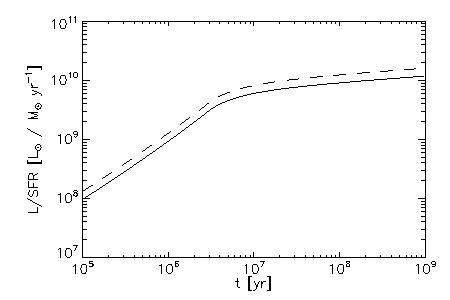
\includegraphics[width=\linewidth]{graphics/hw1sol1}
\caption[Solution to Problem Set~\thesolutionset, Problem~\theenumi\theenumii]{
\label{fig:hw1sol1}
Luminosity normalized by star formation rate for a normal IMF (solid line) and a top-heavy IMF (dashed line).
}
\end{figure}

\item To generate this IMF, I told starbust99 to use a 1 section IMF with a slope of $-2.3$ running from 0.5 to 100 $\msun$. At equal ages, the numbers change to
\begin{eqnarray*}
\mbox{SFR}[\msun\mbox{ yr}^{-1}] & = & 3.2\times 10^{-44} L_{\rm tot}[\mbox{erg s}^{-1}]\qquad\mbox{(10 Myr)} \\
\mbox{SFR}[\msun\mbox{ yr}^{-1}] & = & 2.1\times 10^{-44} L_{\rm tot}[\mbox{erg s}^{-1}]\qquad\mbox{(100 Myr)} \\
\mbox{SFR}[\msun\mbox{ yr}^{-1}] & = & 1.6\times 10^{-44} L_{\rm tot}[\mbox{erg s}^{-1}]\qquad\mbox{(1 Gyr)}.
\end{eqnarray*}
These are a few tens of percent lower, because the IMF contains fewer low mass stars that contribute little light. The effect is mild, but that is partly because the change in IMF is mild. These results do suggest that the IR to SFR conversion does depend on the IMF.

\end{enumerate}

\end{enumerate}
